\documentclass[11pt]{exam}

\usepackage{amsmath, amssymb, multicol}
\usepackage{graphicx}
\usepackage{textcomp}
\usepackage{chessboard}
\usepackage{tikz}

\def\d{\displaystyle}
\def\b{\mathbf}
\def\R{\mathbf{R}}
\def\Z{\mathbf{Z}}
\def\st{~:~}
\def\bar{\overline}
\def\inv{^{-1}}


\newcommand{\vtx}[2]{node[fill,circle,inner sep=0pt, minimum size=4pt,label=#1:#2]{}}
\newcommand{\va}[1]{\vtx{above}{#1}}
\newcommand{\vb}[1]{\vtx{below}{#1}}
\newcommand{\vr}[1]{\vtx{right}{#1}}
\newcommand{\vl}[1]{\vtx{left}{#1}}
\renewcommand{\v}{\vtx{above}{}}


%\pointname{pts}
\pointsinmargin
\marginpointname{pts}
\addpoints
\pagestyle{head}
%\printanswers

\firstpageheader{Math 228}{\bf Review Questions}{Fall 2018}


\begin{document}

%space for name
%\noindent {\large\bf Name:} \underline{\hspace{2.5in}}
%\vskip 1em





\noindent The following questions are meant to remind you about some of the most important topics covered this semester and stimulate you to study the corresponding topics further.  This is NOT a complete list of the things you should know for the final, just a few ideas to get you started.


\begin{questions}
	\question Suppose you were curious about the following statement in graph theory: ``If $G_1$ is bipartite and $G_2$ is isomorphic to $G_1$, then $G_2$ has an even number of edges.''
	\begin{parts}
		\part How would you start a proof of this statement using each of our proof styles?
		\part Use a truth table to help you find a counterexample.
	\end{parts}
	
	\begin{solution}
		\begin{parts}
			\part For a direct proof: Let $G_1$ and $G_2$ be graphs, and assume that $G_1$ is bipartite and that $G_2$ is isomorphic to $G_1$.  (You would then need to prove that $G_2$ has an even number of edges.)
			
			For a proof by contrapositive: Let $G_1$ and $G_2$ be graphs, and assume that $G_2$ does not have an even number of edges.  (You would then need to prove that \emph{either} $G_2$ is not isomorphic to $G_1$ or that $G_1$ is not bipartite, so you could also assume that $G_1$ is isomorphic to $G_2$, and then try to prove that $G_1$ is not bipartite).
			
			For a proof by contradiction: Assume this was not the case.  That is, assume that there are graphs $G_1$ and $G_2$ such that $G_1$ is bipartite, that $G_2$ is isomorphic to $G_1$, and that $G_2$ does NOT have an even number of edges.  (The goal then is any contradiction.)
			
			For proof by induction: Let $P(n)$ be the statement, ``For all graphs $G_1$ and $G_2$ with $n$ vertices, if $G_1$ is bipartite and $G_2$ is isomorphic to $G_1$, then $G_2$ has an even number of vertices.''
			
			You would not do a combinatorial proof of this fact.
			
			\part Make a truth table for the statement $(B \wedge I) \rightarrow E$.  There is only one row in which this evaluates to false: when $B$ is true, $I$ is true, and $E$ is false.  Thus we would be looking for an example of graphs $G_1$ and $G_2$ which are isomorphic and for which $G_1$ is bipartite, but for which $G_2$ does not have an even number of edges.  The simplest such example is the graph $P_2$ (two vertices with 1 edge) for both $G_1$ and $G_2$ (note that if $G_1 = G_2$, then they are definitely isomorphic).
		\end{parts}
	\end{solution}
	
	\question A dodecahedron is a regular convex polyhedron made up of 12 regular pentagons.
	\begin{parts}
	\part Suppose you color each pentagon with one of three colors.  Prove that there must be two adjacent pentagons colored identically.

	\part What if you use four colors?

	\part What if instead of a dodecahedron you colored the faces of a cube?
	\end{parts}


		\begin{solution}
			For all these questions, we are really coloring the vertices of a graph.  You get the graph by first drawing a planar representation of the polyhedron and then taking its \emph{planar dual}: put a vertex in the center of each face (including the outside) and connect two vertices if their faces share an edge.
			\begin{parts}
				\part Since the planar dual of a dodecahedron contains a 5-wheel, it's chromatic number is at least 4.  Alternatively, suppose you could color the faces using 3 colors without any two adjacent faces colored the same.  Take any face and color it blue.  The 5 pentagons bordering this blue pentagon cannot be colored blue.  Color the first one red.  Its two neighbors (adjacent to the blue pentagon) get colored green.  The remaining 2 cannot be blue or green, but also cannot both be red since they are adjacent to each other.  Thus a 4th color is needed.
				\part The planar dual of the dodecahedron is itself a planar graph.  Thus be the 4-color theorem, it can be colored using only 4 colors without two adjacent vertices (corresponding to the faces of the polyhedron) being colored identically.
				\part The cube can be properly 3-colored.  Color the ``top'' and ``bottom'' red, the ``front'' and ``back'' blue, and the ``left'' and ``right'' green.
			\end{parts}
		\end{solution}
	\vfill


	%
	% \question Is it possible to draw a single curve without lifting up your pencil that crosses every line segment below exactly once?  Including the ``outside'' segments?  Explain.
	%
	% \begin{center}
	% \begin{tikzpicture}[xscale=.6]
	% \draw (0,0) rectangle (1.5,1) rectangle (4.5,0) rectangle (6,1) rectangle (3,2) rectangle (0,1);
	% \end{tikzpicture}
	% \end{center}
	%
	% \begin{solution}
	% If we just consider the ``inside'' segments, then it is possible.  Start in the top room and make a ``W''.  This is possible because the top two rooms have three walls (odd number) and the bottom all have even numbers of walls.
	%
	% If we include the outside walls, this is impossible.  Consider the graph you get by placing a vertex in each room, plus a vertex on the ``outside'' with edges connecting vertices if their regions share a wall.  This graph will have 4 vertices with odd degree, so there is no Euler path.
	% \end{solution}


	\question Edward A. Mouse has just finished his brand new house.  The floor plan is shown below:

	\begin{center}
	  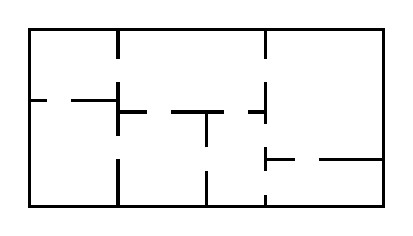
\begin{tikzpicture}[scale=.75]
	    \draw[very thick] (-3,0) rectangle (3,3);
	    \draw[very thick] (-3,1.8) --(-2.7,1.8) (-2.3,1.8) -- (-1.5, 1.8) (-1.5, 1.6) -- (-1,1.6) (-.6, 1.6) -- (.3,1.6) (.7,1.6) -- (1, 1.6) (1, .8) -- (1.5, .8) (1.9,.8) -- (3,.8);
	    \draw[very thick] (-1.5,0) -- (-1.5, .8) (-1.5, 1.2) -- (-1.5,2.1) (-1.5,2.5) -- (-1.5,3);
	    \draw[very thick] (0,0) -- (0,.6) (0,1) -- (0,1.6);
	    \draw[very thick] (1,0) -- (1,.2) (1,.6) -- (1,1) (1,1.4) -- (1,2.1) (1,2.5) -- (1,3);
	  \end{tikzpicture}
	\end{center}


	Edward wants to give a tour of his new pad to a lady-mouse-friend.  Is it possible for them to walk through every doorway exactly once?  If so, in which rooms must they begin and end the tour? Explain.
	 \begin{solution}
	   Yes, he must start in the top right room and end in the bottom middle room, or vice versa.  This is because those are the two rooms with an odd number of doors.

	   In graph theory terms, if we place a vertex in each room and connect vertices if there is a door between their rooms, we are asking whether the graph has an Euler path.  The number of doors is the degree of the vertex, and a graph has an Euler path if and only if there are two or fewer vertices with odd degree.  In that case, the path must start at one of those odd degree vertices and end at the other.
	 \end{solution}
	
	
	
	\vfill
	
\question How many ways can you select 7 jelly beans from 20 flavors?  There are 4 reasonable ``correct'' answers to this way-too-vague question based on various assumptions you would need to make.  What are the assumptions and what are the answers in each case?

\begin{solution}
We need to decide whether repeated flavors are allowed or not.  We also need to decide whether the order in which we select the jelly beans makes a difference (are we taking handfuls or are we lining them up?).  This leads to the 4 reasonable possibilities.

\begin{itemize}
\item No repeats, handfuls: ${20 \choose 7}$.  We just pick which 7 of the twenty to select.
\item No repeats, lineups: $P(20,7) = 20 \cdot 19 \cdot 18 \cdot 17 \cdot 16 \cdot 15 \cdot 14$.  We first pick one of the 20, then pick one of the 19 remaining, and so on until we have selected 7 beans.
\item Repeats allowed, handfuls: ${26 \choose 7}$.  Stars and bars with 19 bars and 7 stars (we switch between the flavors and put a star down every time we take a bean of the flavor we are currently considering).
\item Repeats allowed, lineups: $20^7$.  Just like the permutation, only now the second bean also has 20 choices since we can repeat the flavor.
\end{itemize}
\end{solution}

\vfill

\question How many ways can you distribute 12 books to 4 boxes?  There are actually more than 20 reasonable interpretations of this question, many of which give different answers, and only some of which are things we have learned to do this semester.  What are some assumptions and corresponding answers we can find?

\begin{solution}
	Some questions to ask yourself: are the books distinct?  Are the boxes distinct?  Can some boxes be empty?  Is there an upper limit to the number of books that will fit in a box?  Does it matter what order we put the books into the boxes? Do we need to distribute all the books? 
	
	Here are a few interesting ones we know how to deal with.  
	\begin{enumerate}
		\item If the books and boxes are distinct and boxes are allowed to be empty, then the answer is $4^{12}$, since we have 4 choices for each book. 
		\item If the books and boxes are distinct, but no box is allowed to be empty, then we must use PIE to remove some of the $4^{12}$ solutions that have empty boxes.  This is just like counting surjective (onto) functions.
		\item We could also insist that no box gets more than one book.  There would be 0 ways to do this, but that is because there are more books than boxes.  This is like counting injective (1-1) functions.  If you do not need to distribute all the books, then you are just picking 4 books to put into 4 boxes, so there are $P(12,4)$ choices for the books (assuming both boxes and books are distinct).  If boxes are not distinct, but books are, then the answer would be $\binom{12}{4}$
		\item Say the books are not distinct, but the boxes are.  If we need to distribute all the books, then this is a stars and bars problem.  If boxes can be empty, the answer is $\binom{15}{3}$, if each box needs a book, the answer is $\binom{11}{3}$.
		\item What if each box can hold at most 3 books, and you must distribute all of them, then in fact, each box must hold exactly 3 books.  There are $\binom{12}{3}$ ways to select the books for the first box, $\binom{9}{3}$ ways to select the books for the second box, $\binom{6}{3}$ ways to select the books for the third box, and $\binom{3}{3} = 1$ way to put the remaining 3 books in the last box.  So the answer is $\binom{12}{3}\binom{9}{3}\binom{6}{3}\binom{3}{3}$.  (This is similar to the questions about counting anagrams.)  What if the boxes were not distinct here?  Then we would be overcounting by $4!$, since there are $4!$ to label the boxes.  So you would take that previous answer and divide by $4!$.
		\item Some verions of the problem we don't know how to solve: what if the order in which the books were stacked in the boxes mattered?  This is hard, although it turns out that the answer would be $P(15,3)$.  What if the books were distinct but the boxes were identical?  It turns out that these versions are really really hard: in general, there is no known closed formula for these sorts of questions. 
	\end{enumerate}
	
\end{solution}


\question How many lattice paths start at $(0,0)$, end at $(5,7)$ and pass through $(1,3)$, $(4,3)$, or both?

\begin{solution}
The paths all have length $12$.  If we don't have to pass through the special points, there are ${12\choose 5}$ paths.  But going through the points, we use the multiplicative principle and PIE.

Through $(1,3)$: ${4 \choose 1}{8\choose 4}$\\
Through $(4,3)$: ${7 \choose 4}{5 \choose 1}$\\
Through both: ${4 \choose 1}{3 \choose 3}{5 \choose 1}$\\

All together: ${4 \choose 1}{8\choose 4} + {7 \choose 4}{5 \choose 1} - {4 \choose 1}{3 \choose 3}{5 \choose 1}$.
\end{solution}


\vfill



\question If $A$ is a set containing $n$ elements, how many different subsets (of all sizes) are there of $A$?  Prove your answer using induction.

	\begin{solution}
		We will prove that there are $2^n$ subsets of $A$.  Note this is the same as ${n\choose 0} + {n \choose 1} + {n \choose 2} + \cdots + {n\choose n}$, but let's prove the simpler expression is what we want (we could then prove the two expressions are equivalent using a combinatorial proof).

		Let $P(n)$ be the statement, ``every set containing $n$ elements has $2^n$ different subsets.''  We will show $P(n)$ is true for all $n \ge 1$.

		\underline{Base case}: Any set with 1 element $\{a\}$ has exactly 2 subsets: the empty set and the set itself.  Thus the number of subsets is $2= 2^1$.  Thus $P(1)$ is true.

		\underline{Inductive case}: Suppose $P(k)$ is true for some arbitrary $k \ge 1$.  Thus every set containing exactly $k$ elements has $2^k$ different subsets.  Now consider a set containing $k+1$ elements: $A = \{a_1, a_2, \ldots, a_k, a_{k+1}\}$.  Any subset of $A$ must either contain $a_{k+1}$ or not.  In other words, a subset of $A$ is just a subset of $\{a_1, a_2,\ldots, a_k\}$ with or without $a_{k+1}$.  Thus there are $2^k$ subsets of $A$ which contain $a_{k+1}$ and another $2^{k+1}$ subsets of $A$ which do not contain $a^{k+1}$.  This gives a total of $2^k + 2^k = 2\cdot 2^k = 2^{k+1}$ subsets of $A$.  But our choice of $A$ was arbitrary, so this works for any subset containing $k+1$ elements, so $P(k+1)$ is true.

		Therefore, by the principle of mathematical induction, $P(n)$ is true for all $n \ge 1$.
	\end{solution}

\vfill


\question Consider the recurrence relation $a_n = 3a_{n-1} - 2a_{n-2}$.
\begin{parts}
\part Does the sequence $1, 2, 4, 8, 16, 32, \ldots$ satisfy the recurrence relation?  Are you sure?
\begin{solution}
While there is a nicer recurrence relation for the powers of 2, this does fit the recurrence relation.  Try it!
\end{solution}

\part Find the closed formula for $a_n$ satisfying the recurrence relation and the initial terms $a_0 = 1$, $a_1 = 5$.

\begin{solution}
We can use characteristic roots.  The characteristic polynomial is $x^2 - 3x + 2$ which has roots $x = 2$ and $x = 1$.  Thus $a_n = b\cdot 2^n + c \cdot 1^n$ for some constants $b$ and $c$.  To find them, we set
\[a_0 = 1 = b + c\]
\[a_1 = 5 = b\cdot 2 + c\]
and find $b = 4$ and $c = -3$.  Thus the closed formula is
\[a_n = 4\cdot 2^n - 3\]
\end{solution}

\part Suppose $a_0 = 1$, $a_1 = 1$.  Prove, using strong induction, that $a_n = 1$ for all $n$.  %Characteristic roots first with different intial conditions?  Then this?  Perhaps make this a word problem?  Maybe paths through graphs?

	\begin{solution}
		Let $P(n)$ be the statement, ``$a_n = 1$.''  We will show that $P(n)$ is true for all $n \ge 0$.  The base case is satisfied because by definition $a_0$ and $a_1$ are 1.  Now suppose $P(k)$ is true for all $k < n$.  What is $a_n$?  It is $3a_{n-1} - 2a_{n-2}$.  By the inductive hypothesis, $a_{n-1} = 1$ and $a_{n-2} = 1$.  Thus
		\[a_n = 3\cdot 1 - 2 \cdot 1 = 1.\]

		Therefore, by the principle of strong mathematical induction, $P(n)$ is true for all $n \ge 0$.
	\end{solution}

\end{parts}


\vfill




\end{questions}

\end{document}
